\chapter{Seven layers}

\section{Introductions}

A group of inter-related protocols necessary to perform a communication function is called a \textbf{protocol suite}.The \textbf{TCP/IP protocol suite} is an open standard, meaning these protocols are freely available to the public, and any vendor is able to implement these protocols on their hardware or in their software. The TCP/IP protocol suite includes many protocols, as shown in Figure \ref{TCPIP}.

\begin{figure}[hbtp]
\caption{TCP/IP protocol suite and Communication process}\label{TCPIP}
\centering
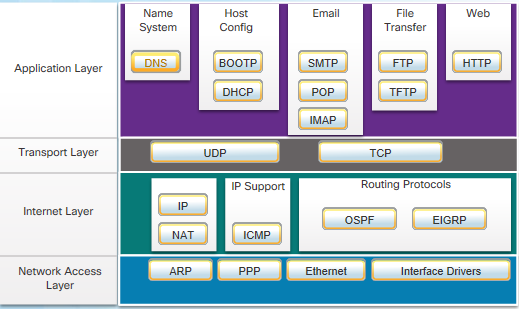
\includegraphics[scale=0.7]{pictures/TCPIP.PNG}
\end{figure}

Figure \ref{ProtocolEncap}  demonstrate the complete protocol encapsulation during the \textbf{TCP/IP communication process}. The process begins with the web server preparing the HTML page as \emph{data} to be sent. The application protocol \emph{HTTP} header is added to the front of the HTML data. The transport layer divides a data stream into segments and may add reliability and flow control information (TCP). Next, the Layer 3 (network layer) adds IP addresses and control information to each segment to create packets. Then, Layer 2 (Data Link layer) protocol (Ethernet, PPP, HDLC, etc.) adds information to both ends of the IP packet, known as a data link frame. This data is now ready to be transported through the internetwork via Layer 1 (Physical layer).\\

\begin{figure}[hbtp]
\caption{Protocol encapsulation}\label{ProtocolEncap}
\centering
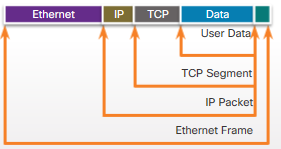
\includegraphics[scale=0.8]{pictures/ProtocolEncap.PNG}
\end{figure}

Whereas the TCP/IP model layers (table \ref{TCP}) are referred to only by name, the seven OSI model layers (table \ref{OSI}) are more often referred to by number rather than by name. For instance, the physical layer is referred to as Layer 1 of the OSI model.

\tableStart[\caption{The OSI Reference Model}\label{OSI}] {|cl p{12cm}|}
\head{Number} & \head{Layer} & \head{Description} \w
7 & Application & contain protocols used for process-toprocess communications\w
6 & Presentation & provide for common representation of the data transferred between application layer services\w
5 & Session & organize dialog and manage data exchange\w
4 & Transport & segment, transfer, and reassemble\w
3 & Network & exchange the individual pieces of data over the network \w
2 & Data Link & exchange data frames between devices over a common media\w
1 & Physical & describe the mechanical, electrical media to create physical connections for bit transmission\w
\tableEnd

\tableStart[\caption{The TCP/IP Reference Model}\label{TCP}] {|c|p{12cm}|}
\head{Layer} & \head{Description} \w
Application & represent data to user plus encoding and dialog control\w
Transport & support communication between various devices across diverse networks\w
Internet & determine best path through the network \w
Network Access & control hardware devices and media\w
\tableEnd

\section{Physical layer}

\subsection{Introduction}

The OSI physical layer provides the means to transport the bits that make up a data link layer frame across the network media. This layer accepts a complete frame from the data link layer and encodes it as a series of signals that are transmitted onto the local media.\\

The physical layer standards address three functional areas:

\begin{itemize}
\item \textbf{Physical Components:} electronic hardware devices, media, and other connectors that transmit and carry the signals to represent the bits.

\item \textbf{Encoding:} a method of converting a stream of data bits into a predefined code. Codes are groupings of bits used to provide a predictable pattern that can be recognized by both the sender and the receiver. 

\item \textbf{Signaling:} The physical layer must generate the electrical, optical, or wireless signals that represent the 1 and 0 on the media. The method of representing the bits is called the \emph{signaling method}. A common signaling method  is using modulation techniques. \emph{Modulation} is the process by which the characteristic of one wave (the signal) modifies another wave (the carrier).
\end{itemize}

\textbf{Bandwidth} is the capacity of a medium to carry data. Digital bandwidth measures the amount of data that can flow from one place to another in a given amount of time in kb/s, Mb/s, and Gb/s. A combination of factors determines the practical bandwidth of a network: The properties of the physical media, The technologies chosen for signaling and detecting network signals.\\

\textbf{Throughput} is the measure of the transfer of bits across the media over a given period of time. Due to a number of factors, throughput usually does not match the specified bandwidth in physical layer implementations. Many factors influence throughput, including: The type and amount of traffic and Latency\footnote{Latency refers to the amount of time, to include delays, for data to travel from one given point to another.} between source and destination. \emph{Throughput cannot be faster than the slowest link in the path from source to destination}. \\

There are three basic forms of network media: Copper cable (electrical pulses), fiber optic (light), and wireless (microwave transmissions).\\

\subsection{Copper cable}

Copper cable is inexpensive and easy to install but limited by distance and signal interference. There are two sources of signal interference:

\begin{itemize}
\item \textbf{EMI or RIF:} distort and corrupt the data signals; potential source: radio waves, electromagnetic devices, such as fluorescent lights or electric motors. To counter the negative effects of EMI and RFI, some types of copper cables are wrapped in metallic shielding and require proper grounding connections.

\item \textbf{Crosstalk} is a disturbance caused by the electric or magnetic fields of a signal on one wire to the signal in an adjacent wire. To counter the negative effects of crosstalk, some types of copper cables have opposing circuit wire pairs twisted together. 
\end{itemize}

There are three main types of copper media used in networking:

\begin{itemize}
\item \textbf{Unshielded Twisted-Pair (UTP):} These cables are used to interconnect nodes on a LAN and infrastructure devices such as PCs, switches, routers. UTP cabling, terminated with \textbf{RJ-45} connectors, consists of \textbf{four} pairs of color-coded wires that have been twisted together. 

\item \textbf{Shielded twisted-pair (STP)} provides better noise protection than UTP cabling.

\item \textbf{Coaxial cable} contains two conductors that share the same axis. 
\end{itemize}

\tableStart[\caption{UTP Categories}\label{UTPcat}] {|l|l|}
\head{Category} & \head{Speed} \w
Cat3 Cable (UTP) & 10Mb/s\w
Cat5 & 100 -- 1000 Mb/s\w
Cat5e& 1000 Mb/s \w
Cat6 &  1000 Mb/s -- 10 Gb/s \w
\tableEnd

\tableStart[\caption{Copper cable types}] {|l|p{4cm}|p{10cm}|}
\head{UTP cable} & \head{Standard} & \head{Application} \\
Straight-through & Both ends T568A or T568B & PC to switch, switch to router \w
Crossover & One end T568A, the other end T568B & switch to switch, router to router, PC to router \w
Rollover & Cisco proprietary & Connects a workstation serial port to a router console port \w
\tableEnd

\subsection{Fiber optic}

Optical fiber cable transmits data over longer distances and at higher bandwidths than any other networking media. Unlike copper wires, fiber-optic cable can transmit signals with less attenuation and is completely immune to EMI and RFI. 

\tableStart[\caption{Fiber Cable Components}]{|l|p{12cm}|
\head{Component} & \head{Description} \w
Core & The core is actually the light transmission element at the center of the optical fiber. This core is typically silica or glass. Light pulses travel through the fiber core.\w
Cladding & It tends to act like a mirror by reflecting light back into the core of the fiber. This keeps light in the core as it travels down the fiber.\w
Buffer & Used to help shield the core and cladding from damage.\w
Strengthening material & Surrounds the buffer, prevents the fiber cable from being stretched when it is being pulled. The material used is often the same material used to produce bulletproof vests.\w
Jacket & a PVC jacket that protects the fiber against abrasion, moisture, and other contaminants.\w
\tableEnd

Light pulses representing the transmitted data as bits on the media are generated by either Lasers or LEDs. Fiber-optic cables are broadly classified into two types:

\begin{itemize}
\item \textbf{Single-mode fiber (SMF)} consists of a very small core and uses \emph{laser} to send a \emph{single} ray of light. Popular in long-distance situations spanning hundreds of kilometers: long-haul telephony, cable TV, campus backbones .

\item \textbf{Multimode fiber (MMF)} consists of a larger core and uses LED emitters to send light pulses. It provides bandwidth up to 10 Gb/s over link lengths of up to 550 meters.

\item One of the highlighted differences between multimode and single-mode fiber is the amount of \emph{dispersion}. Dispersion refers to the spreading out of a light pulse over time. The more dispersion there is, the greater the loss of signal strength.
\end{itemize}

\subsection{Wireless}

Wireless media provides the greatest mobility options of all media. Wireless does have some areas of concern, including Coverage area, Interference, Security, and Shared medium. There are many types of wireless media: WiFi (IEEE 802.11 standard), Bluetooth  (IEEE 802.15 standard), and Wi Max (IEEE 802.16 Standard).

\section{Data Link layer}

The PDU of Data Link layer is always \textbf{frame}. The data link layer is divided into two sublayers: Logical Link Control (LLC) and Media Access Control (MAC). See Figure \ref{Sublayers}.

\subsection{Logical Link Control sublayer (LLC)}

This upper sublayer communicates with the network layer. It places information in the frame that identifies which network layer protocol is being used for the frame. This information allows multiple Layer 3 protocols, such as IPv4 and IPv6, to utilize the same network interface and media.\\

\begin{figure}[hbtp]
\caption{Data Link sublayers}\label{Sublayers}
\centering
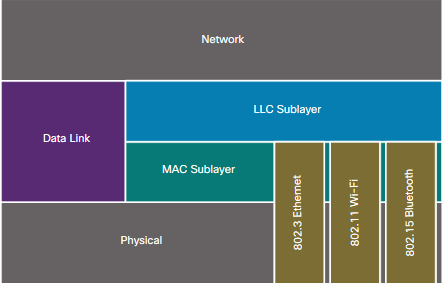
\includegraphics[scale=0.7]{pictures/Sublayers.PNG}
\end{figure}

LLC is implemented in software, and its implementation is independent of the hardware. In a computer, the LLC can be considered the driver software for the NIC. The NIC driver is a program that interacts directly with the hardware on the NIC to pass the data between the MAC sublayer and the physical media.

\subsection{Ethernet MAC sublayer}

The Ethernet MAC sublayer has two primary responsibilities: Data encapsulation and Media Access Control. \\

The \textbf{data encapsulation} process includes frame assembly before transmission and frame disassembly upon reception of a frame. Data encapsulation provides three primary functions: Frame delimiting, Addressing, and Error detection. \\

\textbf{Media access control} is responsible for the placement of frames on the media and the removal of frames from the media. As its name implies, it controls access to the media. This sublayer communicates directly with the physical layer. The actual media access control method used depends on Topology and Media sharing.\\

\paragraph{Multi-access networks} Ethernet LANs\footnote{Various hosts connect to a single switch (or hub) using Ethernet cables.} and WLANs\footnote{Various hosts connect to an access point via radio transmissions} are examples of a multiaccess network. At any one time, there may be a number of devices attempting to send and receive data using the same network media. Therefore, multi-access networks require rules to govern how devices share the physical media. Those rules, together, form a media access control method. There are two basic access control methods for shared media:

\begin{itemize}
\item \textbf{Contention-based access:} All nodes operating in half-duplex compete, only one device can send at a time. Ethernet LANs \emph{using hubs} and WLANs are examples of this type of access control.

\item \textbf{Controlled access:} Each node has its own time to use the medium, a device must wait its turn to access the medium. Legacy Token Ring LANs are an example of this type of access control. 
\end{itemize}

\note Ethernet LANs using \emph{switches} do not use a contention-based system because the switch and the host NIC operate in full-duplex mode.\\

The \textbf{CSMA/CD} (Carrier Sense Multiple Access/Collision Detection) process is used in \emph{half-duplex Ethernet LANs}. A PC's NIC needs to determine if anyone is transmitting on the medium. If it does not detect a carrier signal or receives transmissions from another device, it will assume the network is available to send. If another device wants to transmit, it must wait until the channel is clear. Additionally, CSMA/CD stops transmitting when congestion occurs. It also uses a random time to re-sent a frame.\\

The \textbf{CSMA/CA} (Carrier Sense Multiple Access/Collision Avoidance) process is used in \emph{WLAN}. CSMA/CA does not detect collisions but attempts to avoid them by waiting before transmitting. Each device that transmits includes the time duration that it needs for the transmission. All other wireless devices receive this information and know how long the medium will be unavailable. 

\subsection{Frame}

\subsubsection{Generic Frame}

The data link layer prepares a packet for transport across the local media by encapsulating it with a header and a trailer to create a frame. Each frame has three parts: Header, Data, and Trailer (Figure \ref{Frame}). The generic frame field types include:

\begin{figure}[hbtp]
\caption{Frame fields}\label{Frame}
\centering
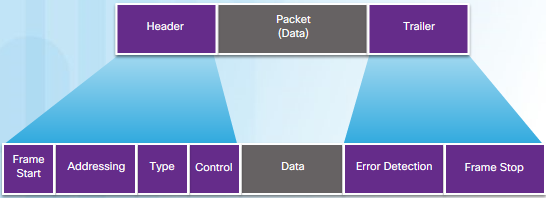
\includegraphics[scale=0.8]{pictures/Frame.PNG}
\end{figure}


\begin{itemize}
\item \textbf{Frame start and stop indicator flags} identify the beginning and end limits of the frame.

\item \textbf{Addressing} indicates the source and destination nodes on the media.

\item \textbf{Type} identifies the Layer 3 protocol in the data field.

\item \textbf{Control} identifies special flow control services such as quality of service (QoS). 

\item \textbf{Data} contains the frame payload 

\item \textbf{Error Detection}
\end{itemize}

The trailer is used to determine if the frame arrived without error. This process is called error detection. Cyclic Redundancy Check (CRC) value is placed in the Frame Check Sequence (FCS) field to represent the contents of the frame. In the Ethernet trailer, the FCS checks transmission errors.\\

\begin{figure}[hbtp]
\caption{Layer 2 Data Link addresses change at each point along the way}\label{Frame2}
\centering
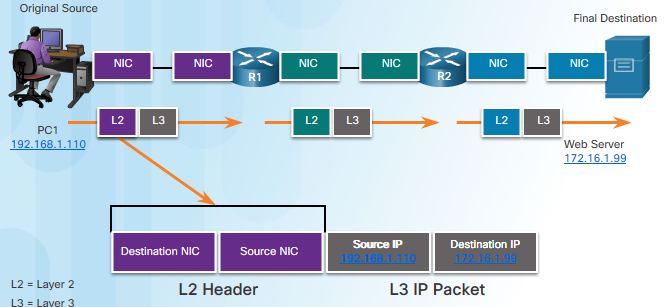
\includegraphics[ width=0.8\textwidth ]{pictures/Frame2.PNG}
\end{figure}

As the IP packet travels from host-to-router, router-to-router, and finally router-to-host, at each point along the way the IP packet is encapsulated in a new data link frame (Figure \ref{Frame2}). Each data link frame contains the source data link address of the NIC card sending the frame and the destination data link address of the NIC card receiving the frame. Remember that the data link layer address is only used for local subnet delivery. 

\subsubsection{Ethernet Frame}

\paragraph{Size} The minimum Ethernet frame size is 64 bytes and the maximum is 1518 bytes\footnote{ The Preamble field is not included when describing the size of a frame.}. Any frame less than 64 bytes in length is called a \emph{collision fragment} or \emph{runt frame}. Frames with more than 1500 bytes of data are called \emph{jumbo frames} or \emph{baby giant frames}. If the size of a transmitted frame is less than the minimum or greater than the maximum, the receiving device drops the frame. 

\paragraph{Frame fields} The \emph{Preamble} (7 bytes) and \emph{Start Frame Delimiter} (1 byte) fields are used for synchronization between the sending and receiving devices. The \emph{Type} field (2 bytes) identifies the upper layer protocol in hexadecimal: IPv4 = 0x800, IPv6 = 0x86DD, ARP = 0x806.

\paragraph{Ethernet MAC addresses}(6 bytes) are made up of two parts: vendor code OUI (3 bytes) assigned by IEEE and device identifier (3 bytes). When the computer starts up, the first thing the NIC does is copy the MAC address from ROM into RAM. \textbf{Broadcast MAC} address is \textbf{FF-FF-FF-FF-FF-FF} (twelve F letters). The \textbf{multicast MAC} address associated with an IPv4 multicast address is a special value that begins with \textbf{01-00-5E} in hexadecimal. The remaining portion of the multicast MAC address is created by converting the lower 24 bits of the IP multicast group address into 6 hexadecimal characters. For an \textbf{IPv6} address, the multicast MAC address begins with \textbf{33-33}.



\subsection{ARP}

To determine the destination MAC address, the device uses ARP. ARP provides two basic functions: Resolving IPv4 addresses to MAC addresses, Maintaining a table of mappings. \\

When a packet is sent to the data link layer to be encapsulated into an Ethernet frame, the device refers to a table in its memory to find the MAC address that is mapped to the IPv4 address. This table is called the ARP table or the ARP cache. The ARP table is stored in the RAM of the device. \\

The sending device will search its ARP table for a destination IPv4 address and a corresponding MAC address. If the destination IPv4 address is on the \emph{same} network as the source IPv4 address, the device will search the ARP table for the destination IPv4 address. Otherwise, the device will search the ARP table for the IPv4 address of the default gateway.\\

For each device, an ARP cache timer removes ARP entries that have not been used for a specified period of time. The times differ depending on the device's operating system. For example, Windows store ARP cache entries for 2 minutes.\\

\paragraph{ARP request} If there is no entry is found in ARP table for a particular IPv4 address, then the device sends an ARP request. ARP messages are encapsulated directly within an Ethernet frame. There is no IPv4 header (Figure \ref{ARPrequest}). Destination MAC address is a broadcast address. ARP messages have a type field of \textbf{0x806}. 

\tableStart[\caption{ARP request message}\label{ARPrequest}] {|c|c|c|c|}
Destination MAC & Source MAC & \textbf{Target} IPv4 & Target MAC \w
FF-FF & 00-0A & 192.68.1.5 & -- \w
\tableEnd

\paragraph{ARP reply} Only the device with an IPv4 address associated with the target IPv4 address in the ARP request will respond with an ARP reply. Only the device that originally sent the ARP request will receive the unicast ARP reply. The ARP reply is encapsulated in an Ethernet frame (Table \ref{ARPreply}).

\tableStart[\caption{ARP request message}\label{ARPreply}] {|c|c|c|c|}
Destination MAC & Source MAC & \textbf{Sender} IPv4 & Sender MAC \w
00-0A & 00-0B & 192.68.1.5 & 00-0B \w
\tableEnd

\paragraph{ARP broadcasts}  If a large number of devices were to be powered up, and all start sending ARP requests, there could be some reduction in performance for a short period of time. 

\paragraph{ARP spoofing} is a technique used by an attacker to reply to an ARP request for an IPv4 address belonging to another device, such as the default gateway. The attacker sends an ARP reply with its own MAC address. The receiver of the ARP reply will add the wrong MAC address to its ARP table and send these packets to the attacker.

\section{Network layer}

Network Layer PDU Is an \textbf{Packet}.

\subsection{Introduction}

The network layer has four basic processes: Addressing end devices, routing, encapsulation, de-encapsulation. There are several network layer protocols in existence, but there are only two network layer protocols that are commonly implemented: \textbf{IPv4} and \textbf{IPv6}.\\

IP encapsulates the transport layer segment or other data by adding an IP header. This header remains the same from the time the packet leaves the source host until it arrives at the destination host.\\

The protocols in network layer were not designed to track and manage the flow of packets. The basic characteristics of IP are

\begin{itemize}
\item \textbf{Connectionless:} no dedicated end-to-end connection is created before data is sent. 
\item \textbf{Best Effort:} The IP protocol does not guarantee that all packets that are received. Furthermore, IP is unreliable which means that IP does not have the capability to manage and recover from undelivered or corrupt packets
\item \textbf{Media Independent:} Operation is independent of the medium (i.e., copper, fiber optic, or wireless) carrying the data.
\end{itemize}

There is, however, one major characteristic of the media that the network layer considers: \textbf{MTU} (maximum transmission unit). The data link layer passes the MTU value up to the network layer. The network layer then determines how large packets can be.\\

Sometimes, a IPv4 router must split up a packet when forwarding it from one medium to another medium with a smaller MTU. This process is called \textbf{fragmentation}. Unlike IPv4, IPv6-enabled routers do not fragment packets.

\subsection{Packet header}

Significant fields in the \textbf{IPv4} header include (Figure \ref{IPv4packet}):

\begin{itemize}
\item \textbf{Version:} is set to \textbf{0100} that identifies this as an IP version 4 packet.

\item \textbf{DiffServ:} used by QoS service to determine the priority.

\item \textbf{TTL:} limit the lifetime of a packet. The value is decreased by one each time the packet is processed by a router. If the TTL field decrements to zero, the router discards the packet and sends an \emph{ICMP Time Exceeded} message to the source IP address.

\item \textbf{Protocol:} identify the next level protocol. Common values include \textbf{ICMP (1)}, \textbf{TCP (6)}, and \textbf{UDP (17)}.

\item \textbf{Source IPv6 Address}

\item \textbf{Destination IPv6 Address}
\end{itemize}

\begin{figure}[hbtp]
\caption{IPv4 packet header}\label{IPv4packet}
\centering
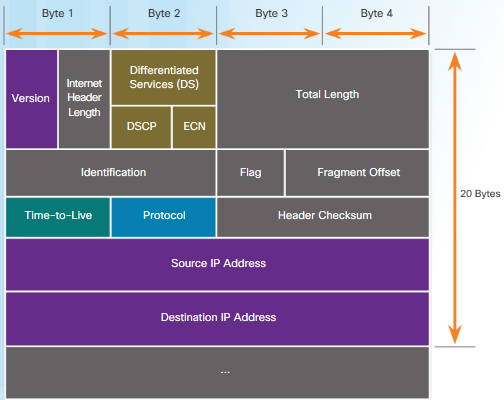
\includegraphics[scale=0.6]{pictures/IPv4packet.PNG}
\end{figure}

Significant fields in the \textbf{IPv6} header include (Figure \ref{IPv6packet}):

\begin{itemize}
\item \textbf{Version:} is set to \textbf{0110} that identifies this as an IP version 6 packet.

\item \textbf{Traffic class:} equivalent to the IPv4 DiffServ field.

\item \textbf{Payload Length:} indicates the length of the data portion of the packet.

\item \textbf{Hop Limit:} equivalent to the IPv4 TTL field.

\item \textbf{Next Header:} equivalent to the IPv4 Protocol field.
\end{itemize}

\subsection{Routing table}

When a router interface (g0/0) is configured with an IPv4 address (192.168.10.1), a subnet mask (255.255.255.0), and is activated, the following two routing table entries are automatically created:

\begin{verbatim}
C 192.168.10.0/24 is directly connected, GigabitEthernet0/0
L 192.168.10.1/32 is directly connected, GigabitEthernet0/0
\end{verbatim}

The letter \textbf{C} identifies a directly connected \emph{network}. The letter \textbf{L} shows that this is a local interface and its IP address is 192.168.10.1.\\

The routing table also stores information about remote network. For example, the entry for the remote network 10.1.1.0 is as follows:

\begin{verbatim}
D 10.1.1.0/24 [90/2170112] via 209.165.200.226, 00:00:09, Serial0/0/0
\end{verbatim}

The details of the remote network routing table entry are explained as follow:

\begin{itemize}
\item \verb|D| -- Identifies how the network was learned by the router. Common  route sources include \textbf{S} (static route), \textbf{D} (EIGRP), \textbf{O} (OSPF).

\item \verb|10.1.1.0/24| -- Identifies the destination network.

\item \verb|90| -- Identifies the AD of the route.

\item \verb|2170112| -- Identifies the metric of the route.

\item \verb|209.165.200.226| -- Identifies the IP address of the router to forward the packet.

\item \verb|00:00:09| -- Router timestamp

\item \verb|Serial0/0/0| -- Identifies the exit interface to use to forward a packet
\end{itemize}

\subsection{Router Boot-up}

This topic will introduce the structure of Cisco routers and how they boots up.\\

A Cisco router has four types of memory:

\begin{itemize}
\item \textbf{RAM:} This is volatile memory that stores: IOS image, Running configuration file, Routing table, ARP cache, and Packet buffer.

\item \textbf{ROM:} This non-volatile memory is used to store Bootstrap program, Power-on self-test (POST), and Limited IOS (backup IOS).

\item \textbf{NVRAM:} This non-volatile memory is used to store Startup configuration file.

\item \textbf{Flash:} This non-volatile computer memory used as permanent storage for the IOS and other system-related files (log, HTML files, etc.) When a router is rebooted, the IOS is copied from flash into RAM.
\end{itemize}

\begin{figure}[hbtp]
\caption{Cisco router bootup process}\label{BootUp}
\centering
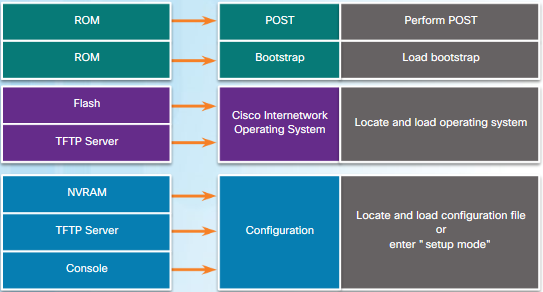
\includegraphics[ width=0.7\textwidth ]{pictures/BootUp.PNG}
\end{figure}

There are three major phases to the bootup process, as shown in Figure \ref{BootUp}.

\begin{enumerate}
\item \textbf{POST process and Bootstrap Program:} During the Power-On Self-Test (POST), the router executes diagnostics on hardware components (CPU, RAM, NVRAM, etc.). After the POST, the bootstrap program is copied from ROM into RAM.

\item \textbf{Loading Cisco IOS:} The IOS image is copied from Flash memory into RAM. If the image is not located in flash, then the router may look for it using a TFTP server. If a full IOS image cannot be located, a Limited IOS (in ROM) is copied into RAM, which can be used to diagnose problems and transfer a full IOS into Flash memory.

\item \textbf{Loading the Startup configuration File:} The bootstrap program then copies the startup configuration file from NVRAM into RAM. This becomes the running configuration. If the startup configuration file does not exist in NVRAM, the router may be configured to search for a TFTP server. If a TFTP server is not found, then the router displays the setup mode prompt.
\end{enumerate}

\note Setup mode is not used in this course to configure the router. When prompted to enter setup mode, always answer no. If you answer yes and enter setup mode, press Ctrl+C at any time to terminate the setup process.\\

Use \verb|show version| to check the version of the Cisco IOS, the version of the bootstrap program, and information about the hardware configuration, including the amount of system memory.

\subsection{Router configuration}

\tableStart[\caption{Initial router configuration}] {|l|l|}
\head{Task} & \head{Commands}\w
Configure the device name & \verb|hostname BranchRouter| \w

Secure user EXEC mode & 
\begin{minipage}{4in}
\begin{verbatim}
line console 0
  password cisco12345
  login
\end{verbatim} 
\end{minipage} \w

Secure remote Telnet/SSH access & 
\begin{minipage}{4in}
\begin{verbatim}
line vty 0 4
  password cisco12345
  login
\end{verbatim} 
\end{minipage} \w

Secure privilege EXEC mode & \verb|Router(config)# enable secret password|\w

Secure all passwords & \verb|Router(config)# service password-encryption|\w

Provide legal notification & \verb|Router(config)# banner motd "message"|\w

Save the configuration & \verb|Router# copy run start|\w

Configure the interface & 
\begin{minipage}{3in}
\begin{verbatim}
interface s0/0/0
  ip address 192.168.100.1 255.255.255.0
  description Connect to R1
  no shutdown
\end{verbatim}
\end{minipage}\w

Verify interface configuration & 
\begin{minipage}{3in}
\begin{verbatim}
show interface
show ip interface
show ip interface brief
show ip route
\end{verbatim}
\end{minipage}\w

\tableEnd

\section{Transport layer}

The PDU of transport layer is either \textbf{segment} or \textbf{datagram}. The transport layer is responsible for:

\begin{itemize}
\item Establishing a temporary communication session between two applications and delivering data between them. 
\item Tracking individual conversations
\item Segmenting data and Reassembling segments
\item To pass data streams to the proper applications, transport layer assigns each application an identifier called a \textbf{port number}. 
\end{itemize}

\subsection{TCP}

TCP is considered a reliable, full-featured transport layer protocol, which ensures that all of the data arrives at the destination. However, this requires additional fields in the TCP header which increases the size of the packet and also increases delay. With TCP, there are three basic operations of reliability:

\begin{itemize}
\item Numbering and tracking data segments transmitted 
\item Acknowledging received data
\item Retransmitting any unacknowledged data 
\end{itemize}

TCP has the following features:

\begin{itemize}
\item  \textbf{Connection-oriented:} TCP negotiates and establishes a virtual connection between source and destination devices prior to forwarding any traffic.

\item \textbf{Reliable:} TCP ensures that each segment arrives at the destination. 

\item \textbf{Stateful protocol:} A stateful protocol is a protocol that keeps track of the state of the communication session. 

\item \textbf{Same-Order Delivery:} Because networks may provide multiple routes that can have different transmission rates, data can arrive in the wrong order. By numbering and sequencing the segments, TCP can ensure that these segments are reassembled into the proper order.

\item \textbf{Flow control:} When TCP is aware that these resources are overtaxed, it can request that the sending application reduce the rate of data flow. To accomplish this, the TCP header includes a field called the \emph{window size}.
\end{itemize}

\begin{figure}[hbtp]
\caption{TCP segment}\label{TCPheader}
\centering
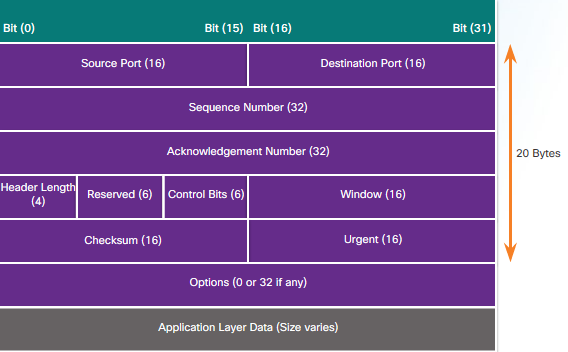
\includegraphics[scale=0.5]{pictures/TCPheader.PNG}
\end{figure}


Each TCP segment has 20 bytes of overhead (Figure \ref{TCPheader}) in the header encapsulating the application layer data:

\begin{itemize}
\item \textbf{Source Port and Destination Port}

\item \textbf{Sequence number} –- Used for data reassembly purposes. During session setup, an \textbf{initial sequence number (ISN)} is set. ISN is the starting value of Sequence number. As data is transmitted during the session, the sequence number is incremented. 

\item \textbf{Acknowledgement number} – Indicates the data that has been received. Acknowledgement number sent back to the source to indicate the next byte that the receiver expects to receive. This is called \emph{expectational acknowledgement}. When TCP at the source host has not received an acknowledgement after a predetermined amount of time, it returns to the last ACK number received and retransmits the data from that point forward. 

\item \textbf{Header length} -– Indicates the length of the TCP segment header.
\item \textbf{Reserved} -– This field is reserved for the future.
\item \textbf{Control bits} -– Known as flags, these identify bit codes that indicate the purpose and function of the TCP segment.
\item \textbf{Window size} -– Indicates the number of bytes that can be accepted at one time. The window size is included in every TCP segment, so the destination can modify the window size at any time depending on buffer availability. The initial window size is agreed upon  TCP three-way handshake. 
\item \textbf{Checksum} -– Used for error checking of the segment header and data.
\item \textbf{Urgent} -– Indicates if data is urgent.
\end{itemize}

A TCP connection is established in three-way handshake:

\begin{enumerate}
\item The client requests a client-to-server communication session with the server
\item The server acknowledges the client-to-server communication session and requests a server-to-client communication session
\item The client acknowledges the server-to-client communication session 
\end{enumerate}

The TCP connect is terminated in \textbf{two} two-way handshakes with four exchanges:

\begin{enumerate}
\item When the client has no more data to send in the stream, it sends a segment with the FIN flag set 
\item The server sends an ACK to acknowledge the receipt of the FIN to terminate the session from client to server. So step 1 and 2 is the first two-way handshake
\item The server sends a FIN to the client to terminate the server-to-client session
\item The client responds with an ACK to acknowledge the FIN from the server
\end{enumerate}

TCP is a \textbf{full-duplex} protocol, where each connection represents two one-way communication sessions. To establish the connection, the hosts perform a \textbf{three-way handshake}. Control bits in the TCP header indicate the progress and status of the connection. 

\subsection{UDP}

UDP is a lightweight transport protocol that offers the same data segmentation and reassembly as TCP, but without TCP reliability and flow control. It is known as a \textbf{best-effort} delivery protocol. UDP is also a \textbf{stateless} protocol, meaning neither the client, nor the server, is obligated to keep track of the state of the communication session.\\

\begin{figure}[hbtp]
\caption{UDP datagram}\label{UDPheader}
\centering
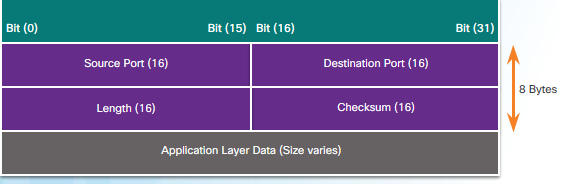
\includegraphics[scale=0.5]{pictures/UDPheader.PNG}
\end{figure}


UDP has no way to reorder the datagrams into their transmission order. Therefore, UDP simply reassembles the data in the order that it was received and forwards it to the application. \\

The pieces of communication in UDP are called datagrams. These datagrams are sent as best-effort by the transport layer protocol. UDP has a low overhead of 8 bytes (Figure \ref{UDPheader}).

There are three types of applications that are best suited for UDP:

\begin{itemize}
\item Live video and multimedia applications (e.g. VoIP, live streaming video)
\item Simple request and reply applications (e.g. DNS\footnote{DNS can also use TCP if the DNS request or DNS response is more than 512 bytes}, DHCP)
\item Applications that handle reliability themselves (SNMP\footnote{SNMP uses UDP by default, but it can also use TCP}, TFTP)
\end{itemize}

\subsection{Port number}

The source port number is associated with the originating application on the local host. The destination port number is associated with the destination application on the remote host. Each application process running on the server is configured to use a port number. An individual server cannot have two services assigned to the same port number within the same transport layer services.\\

The combination of the source IP address and source port number, or the destination IP address and destination port number is known as a socket. The socket is used to identify the server and service being requested by the client. In figure \ref{Socket}, the client socket is 192.168.1.5:1099 with 1099 representing the source number, the socket on the web server is 192.168.1.7:80. Together, these two sockets combine to form a socket pair: 192.168.1.5:1099, 192.168.1.7:80 \\

\begin{figure}[hbtp]
\caption{Examples of socket pairs}\label{Socket}
\centering
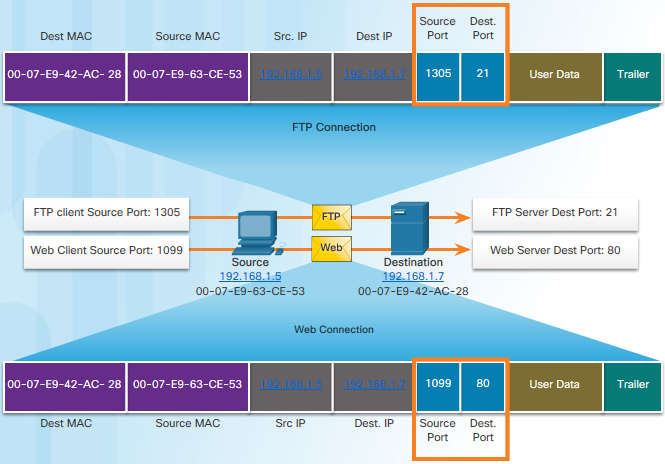
\includegraphics[ width=0.7\textwidth ]{pictures/Socket.PNG}
\end{figure}

There are different types of port numbers:

\begin{itemize}
\item \textbf{Well-known Ports} (0 -- 1023): These numbers are used for popular applications such as FTP, HTTP, TFTP, etc.

\item \textbf{Registered Ports} (1024 -- 49151): These port numbers are assigned by IANA to a requesting entity to use with specific processes or applications.

\item \textbf{Dynamic or Private Ports} (49152 -- 65535): These are assigned dynamically by the client's OS to identify the application during communication.
\end{itemize}

\tableStart[\caption{Protocol port number}] {|l|l|l|}
\head{Port number} & \head{Protocol} & \head{Application}\w
20 & TCP & FTP (data)\w
21 & TCP & FTP (client)\w
22 & TCP & SSH\w
23 & TCP & Telnet\w
25 & TCP & SMTP\w
53 & UDP, TCP & DNS\w
67, 68 & UDP & DHCP\w
69 & UDP & TFTP\w
80 & TCP & HTTP\w
443 & TCP & HTTPS\w
110 & TCP & POP3\w
143 & TCP & IMAP\w
161 & UDP & SNMP\w
\tableEnd

\section{Application layer}

The PDU of application layer is \textbf{data}.  Application layer protocols are used to exchange data between programs running on the source and destination hosts. The upper three layers of the OSI model (application, presentation, and session) define functions of the single TCP/IP application layer.

\subsection{Presentation and Session Layer}

The presentation layer has three primary functions: Formatting, Compressing, and Encrypting. Specifically, it formats data for the application layer, and it sets standards for file formats (QuickTime, MPEG, GIF, PNG, JPEG, etc.).\\

Functions at the session layer create and maintain dialogs between source and destination applications. The session layer handles the exchange of information to initiate dialogs, keep them active, and to restart sessions that are disrupted or idle for a long period of time.\\

\subsection{Peer-to-peer network}

In the peer-to-peer (P2P) networking model, the data is accessed from a peer device without the use of a dedicated server. The P2P network model involves two parts: P2P networks and P2P applications. Every connected end device (known as a peer) can function as both a server and a client. \\

With P2P applications, each computer in the network running the application can act as a client or a server for the other computers in the network running the application. Common P2P networks include: eDonkey, G2, BitTorrent, Bitcoin. Some P2P applications are based on the Gnutella protocol, where each user shares whole files with other users. 

\subsection{HTTP}

When a web address or URL (uniform resource locator) is typed into a web browser, the web browser establishes a connection to the web service running on the server using the HTTP protocol. URLs and URIs (Uniform Resource Identifier) are the names most people associate with web addresses.\\

HTTP is a request/response protocol. When a client sends a request to a web server, HTTP specifies the message types used for that communication. The three common message types are GET (A client request for data), POST (Upload data files), and PUT (Upload resources or content).\\

\textbf{HTTPS} uses the same client request-server response process as HTTP, but the data stream is encrypted with Secure Socket Layer (SSL) before being transported across the network.

\subsection{Email}

Email is a \emph{store-and-forward} method of sending, storing, and retrieving electronic messages across a network. Email messages are stored in databases on mail servers. An email client does not communicate directly with another email client when sending email. Instead, both clients rely on the mail server to transport messages. \\

Email supports three separate protocols for operation: SMTP, POP3, IMAP. The application layer process that sends mail uses SMTP. A client retrieves email using one of the two application layer protocols: POP or IMAP.\\

SMTP port is \textbf{25}. \\

When the server receives the message, it either places the message in a local account (if the recipient is local) or forwards the message to another mail server for delivery. The destination email server may not be online or may be busy when email messages are sent. Therefore, SMTP spools messages to be sent at a later time. Periodically, the server checks the queue for messages and attempts to send them again. If the message is still not delivered after a predetermined expiration time, it is returned to the sender as undeliverable. \\

\paragraph{POP3} is used to retrieve mail from a mail server. With POP, by default, mail is downloaded from the server to the client and then deleted on the server. 

\paragraph{IMAP} is another protocol that describes a method to retrieve email messages. Unlike POP, when the user connects to an IMAP-capable server, copies of the messages are downloaded to the client application.  The original messages are kept on the server until manually deleted. With IMAP, users can create a file hierarchy on the server to organize and store mail. That file structure is duplicated on the email client as well. When a user decides to delete a message, the server synchronizes that action and deletes the message from the server.

\subsection{DNS}

In data networks, devices are labeled with numeric IP addresses to send and receive data over networks. Domain names were created to convert the numeric address into a simple, recognizable name. For example, a domain name, such as \verb|http://www.cisco.com|, is much easier for people to remember than 198.133.219.25, which is the actual numeric address for this server. \\

The DNS (Domain Name Service)  defines an automated service that matches resource names with the required numeric network address. The steps involved in DNS resolution are as follows:

\begin{enumerate}
\item User enters a fully qualified domain name (FQDN).
\item The client computer  sends a DNS query to the DNS server requesting an IP address to match the FQDN
\item The DNS server resolve the FQDN to an IP address in the DNS server database
\item The DNS server sends back a response to the client with the IP address for the FQDN
\end{enumerate}

The DNS server stores different types of resource records used to resolve names. These records contain the name, address, and type of record. Some of these record types are:

\begin{itemize}
\item A – An end device IPv4 address
\item NS – An authoritative name server
\item AAAA – An end device IPv6 address (pronounced quad-A)
\item MX – A mail exchange record
\end{itemize}

When a client makes a query, the server's DNS process first looks at its own records to resolve the name. If it is unable to resolve the name using its stored records, it contacts other servers to resolve the name. After a match is found and returned to the original requesting server, the server temporarily stores the numbered address in the event that the same name is requested again. The DNS Client service on Windows PCs also stores previously resolved names in memory. The \code{ipconfig /displaydns} command displays all of the cached DNS entries.\\

\begin{figure}[hbtp]
\caption{A hierarchy of DNS server}\label{DNSprocess}
\centering
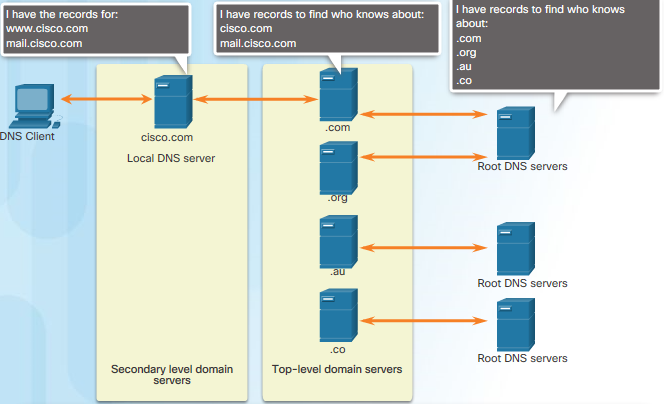
\includegraphics[ width=0.8\textwidth ]{pictures/DNSprocess.PNG}
\end{figure}


The DNS protocol uses a hierarchical system to create a database to provide name resolution (Figure \ref{DNSprocess}). The naming structure is broken down into small, manageable zones. Each DNS server maintains a specific database file and is only responsible for managing name-to-IP mappings for that small portion of the entire DNS structure.\\

The different top-level domains represent either the type of organization or the country of origin. Examples of top-level domains are: .com (business or industry), .org (non-profit organization), .fi (Finland), etc.\\

Computer operating systems also have a utility called \emph{nslookup} that allows the user to manually query the name servers to resolve a given host name. This utility can also be used to troubleshoot name resolution issues and to verify the current status of the name servers. When the nslookup command is issued, the default DNS server configured for your host is displayed. 

\subsection{FTP}

FTP transfers data between a client and a server. To successfully transfer data, FTP requires two connections between the client and the server, one for commands and replies, the other for the actual file transfer:

\begin{itemize}
\item The \textbf{client} establishes the first connection to the server for control traffic using \textbf{TCP} port \textbf{21}, consisting of client \emph{commands} and server \emph{replies}.

\item The client establishes the second connection to the server for the \emph{actual data transfer} using \textbf{TCP} port \textbf{20}. This connection is created every time there is data to be transferred. The data transfer can happen in either direction. The client can download (pull) data from the server, or the client can upload (push) data to the server.
\end{itemize}

\subsection{SMB}

The Server Message Block (SMB) is a client/server file sharing protocol that describes the structure of shared network resources, such as directories, files, printers, and serial ports. It is a request-response protocol. SMB messages can

\begin{itemize}
\item Start, authenticate, and terminate sessions
\item Control file and printer access
\item Allow an application to send or receive messages to or from another device
\end{itemize}

Microsoft support SMB file-sharing. Unlike the file sharing supported by FTP, clients establish a long-term connection to servers. After the connection is established, the user of the client can access the resources on the server as if the resource is local to the client host. The LINUX and UNIX operating systems also provide a method of sharing resources with Microsoft networks using a version of SMB called \emph{SAMBA}. 